\documentclass{article}
\usepackage[utf8]{inputenc}
\usepackage{enumerate}
\usepackage{graphicx}

\title{COL333: Assignment 3}
\author{Sachin 2019CS10722\\ Saurabh Verma 2019CS50129 }
\date{November 2021}

\begin{document}

\maketitle

\section{Part A: Computing Policies}


\subsection{Formulation of the Taxi Domain as an MDP:}

We have created an MDP for the Taxi Domain formulation as described in the problem statement. We take the wall locations, position of depots, and width and height of the grid as input. Then we create an instance of the map class with these values and use in the MDP.
\begin{enumerate}[a)]
    \item
\textbf{State Space:}
We have created a class for the state. Each state in Taxi Driver MDP has four identifying features: the position of the taxi, position of the passenger,a boolean variable picked denoting whether passenger is picked by the taxi, and the destination. These are the variable describing the state.\\
Now the x position can take discrete values up to the width, y position can take up to the height.So the total number of values position of passenger and position of taxi can take is height*width. But when the boolean value of picked is true then position of taxi and passenger is same. And destination variable takes values equal to the number of depots. \\
So that makes the total number of variables to be (width of the map)*(height of the map)*(width of the map)*(height of the map)*(number of depots)+(width of the map)*(height of the map)*(number of depots). This is the state space.\\
\newline
\textbf{Transition Model:}Now the action in our formulation are (N,S,E,W,PICK,DROP). So the transition model is as follows.
\begin{itemize}
    \item T((pos1,pos2,picked,d),DROP,(pos1,pos2,picked,d))=1
    \item T((pos1,pos2,picked,d),PICK,(pos1,pos2,picked,d))=1
\end{itemize}
Suppose the action is N the the transition model is as follows. This same applies to all the other direction.(the x and y values get modified accordingly)
\begin{itemize}
    \item T(((x,y),pos2,picked,d),N,((x,y+1),pos2,picked,d))=0.85
    \item T(((x,y),pos2,picked,d),N,((x,y-1),pos2,picked,d))=0.05
    \item T(((x,y),pos2,picked,d),N,((x-1,y),pos2,picked,d))=0.05
    \item T(((x,y),pos2,picked,d),N,((x+1,y),pos2,picked,d))=0.05
    \item If there exists a wall between two position\\
        T(((x,y),pos2,picked,d),N,((x,y),pos2,picked,d))=0\\
\end{itemize}


\textbf{Reward Model:}The reward structure is as follows:
\begin{itemize}
    \item if pos1=pos2=d\\
    R((pos1,pos2,picked=True,d),DROP,(pos1,pos2,picked=False,d)=10
    \item if pos1!=pos2\\
    R((pos1,pos2,picked,d),PICK,(pos1,pos2,picked,d))=-10
    \item if pos1!=pos2\\
    R((pos1,pos2,picked,d),DROP,(pos1,pos2,picked,d))=-10 if pos1!=pos2 
    \item All other transitions have a reward of -1
\end{itemize}
\end{enumerate}


\subsection{Implementing Value Iteration for the Taxi Domain:}
\begin{enumerate}[a)]
    \item We implemented the policy iteration in our code in the MDP class. The policy iteration took epsilon as the input. Also, the default value of gamma is set to be 0.9 but can be changed as specified. For the epsilon value of 0.1, the number of iteration the code took to converge is 15.
    \item The plot of max norm distance vs iteration index is given as follow: (The discount factors are given in the range [0.01,0.1,0.5,0.8,0.99] in that order)
    \begin{center}
        \begin{figure}[h]
\hfill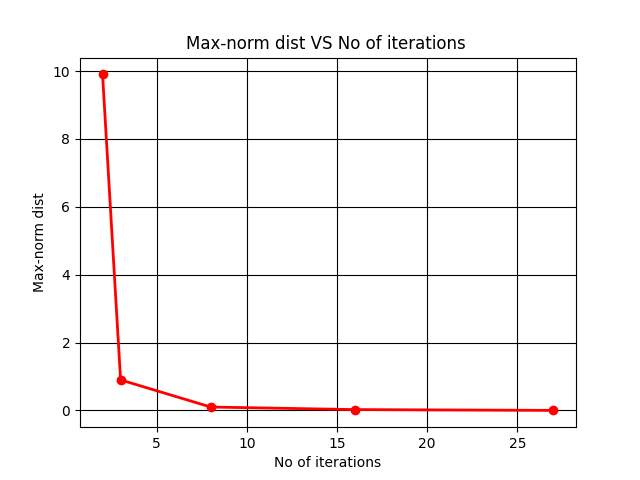
\includegraphics[width=9cm]{QA2b.png}\hspace*{\fill}
        \caption{Max Norm distance vs iteration Index}
        \label{fig:Max Norm distance vs iteration Index}
\end{figure}
\end{center}
    The max-norm distance in a sense signifies the maximum difference from the optimal value. So as the number of iteration of convergence is increasing we are coming more and more close to the optimal value. Our estimates are improving further and further as we increase the number of iterations, hence the max-norm distance decreases. \\
    One another way to look at it is that as the max-norm distance decreases, the estimate value must be close to the optimal value itself, hence the number of iteration of convergence is more. 
    \item
\end{enumerate}
\subsection{Implementing Policy Iteration for the Taxi Domain:}
\begin{enumerate}[a)]
    \item To implement the policy evaluation step, we have two options; one is the exact method in which we create linear equations in variables equal to the number of the total state and get the exact utility value of the various states. The other is the approximate method which runs an update on the states until the value converges.
The first method mentioned is called Linear Algebra Method, the second one is the Iterative method. We have implemented them both. \\
The linear algebra method takes O($n^3$) time for policy evaluation, where n is the number of states. If the transition model given to us is sparse, meaning that each state transition leads to only a small number of states, then the Linear algebra method is preferred because then the solution is obtained faster. The linear Algebra method is preferred when our state space is small. For larger state space, O($n^3$) becomes too much overhead, so iterative method is preferred
    \item The graph comes out as following for different values of the discount factor.
    \begin{center}
        \begin{figure}[h]
\hfill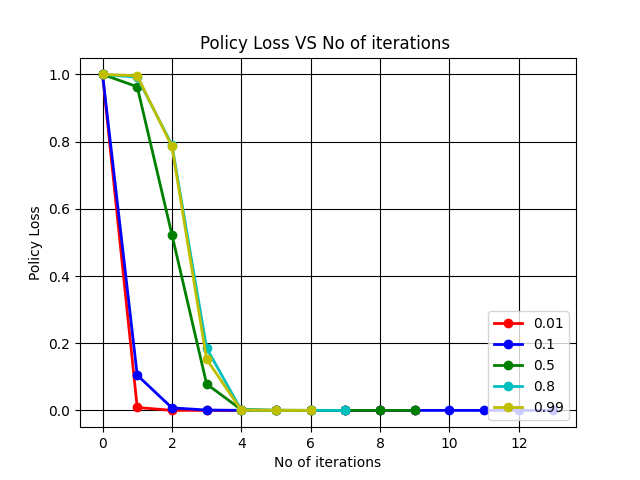
\includegraphics[height=6.5cm]{QA3b.png}\hspace*{\fill}
\end{figure}
\end{center}


\section{Part B: Incorporating Learning}


\subsection{Implementing the approaches to learn the optimal policy:}
In this part we had to implement the Q learning and SARSA reinforcement learning techniques with different exploration methods.\\
For doing that we made a general function that on changing parameter becomes required algorithm. This function takes epsilon and alpha as
parameters and learns the optimal Q table. Initially we started with Q table with all values 0 and performed n number of iterations of episodes. In 
each episode, starting from a random state we keep on moving to next state by performing action depending upon exploration technique and updating Q value depending on
algorithm (Q learning or SARSA) by using the reward got upon performing that action untill we reached terminal state. 
\begin{itemize}
    \item \textbf{Q learning: }  This is an online algorithm, where Q table is updated using the following formula:- 
        $ $
    \item \textbf{SARSA: }  This is an offline algorithm, where Q table is updated using the following formula:- 
        $ $
\end{itemize}

\begin{itemize}
    \item \textbf{e-greedy: } Any random action with probability e otherwise best action according to Q table.
    \item \textbf{exploration decay: } Any random action with probability e/$\sqrt{i}$ (where i = iteration number) otherwise best action according to Q table.
\end{itemize}


\end{enumerate}
\end{document}
